% !TeX root = ../main.tex
% !TeX encoding = UTF-8
% !TeX spellcheck = none

\section{引言}\label{sec:introduction}

准确的交通流量预测是智能交通系统的重要基础，可为主动交通管理、拥堵缓解、路径引导及城市级交通调度提供前瞻性支持。随着深度学习的发展，交通预测已由单变量时间序列分析逐步转向联合刻画空间依赖与时间动态的时空建模框架。DCRNN、STGCN 和 Graph WaveNet 等代表性图模型奠定了基于路网拓扑进行时空联合建模的基本范式 \cite{ref01,ref02,ref03}；随后，ASTGCN、GMAN 等通过注意力机制增强动态相关性建模 \cite{ref04,ref05}，MTGNN、AGCRN 等进一步学习数据驱动的空间关系 \cite{ref06,ref07}，STSGCN 和 STFGNN 则从时空同步建模和多尺度时空融合等角度强化空间交互 \cite{ref08,ref09}。与此同时，PDFormer 引入传播时延感知机制 \cite{ref10}，STWave 利用频率分解区分不同时间动态 \cite{ref11}，PatchTST 和 TimeMixer 等通用时间序列模型则拓展了长程时间依赖建模能力 \cite{ref12,ref13}；对于规则网格上的区域流量，ST-ResNet 和 DeepSTN+ 通过卷积结构建模局部空间模式 \cite{ref14,ref15}。上述研究显著提升了交通流的时空表征能力，也构成了当前交通预测研究的主要技术基础。类似的研究演进在现有综述型工作中也表现为从图结构、注意力、动态图到频率与长序列建模的逐步扩展\cite{ref16,ref17}。

然而，获得更强的时空表征并不等价于能够充分应对交通状态对常规模式的局部偏离。实际交通流在大多数时段呈现较稳定的周期与空间协同规律，但局部区域仍可能出现与常规时段模式不一致的短时变化。当某一区域的近期流量明显偏离其常规时段模式时，未来状态往往同时受到节点自身短时变化以及跨区域历史信息的影响。此时，仅依赖一个统一的时空表示并不足以回答两个更具体的问题：不同类型的预测证据应如何被组织，以及哪些跨区域历史信息在当前状态下真正具有参考价值。

图~\ref{fig:intro-case}以成都网格601的流出量为例，展示了上述现象。同区域既往模式和邻区提前30分钟的观测提供了不同来源的历史参照；即使目标与邻区在历史窗口内高度相关，对齐后的实测后续曲线仍可呈现不同程度的差异。这提示有必要区分证据来源，并结合当前状态和预测时距判断历史信息的适用性。

\begin{figure}[!t]
  \centering
  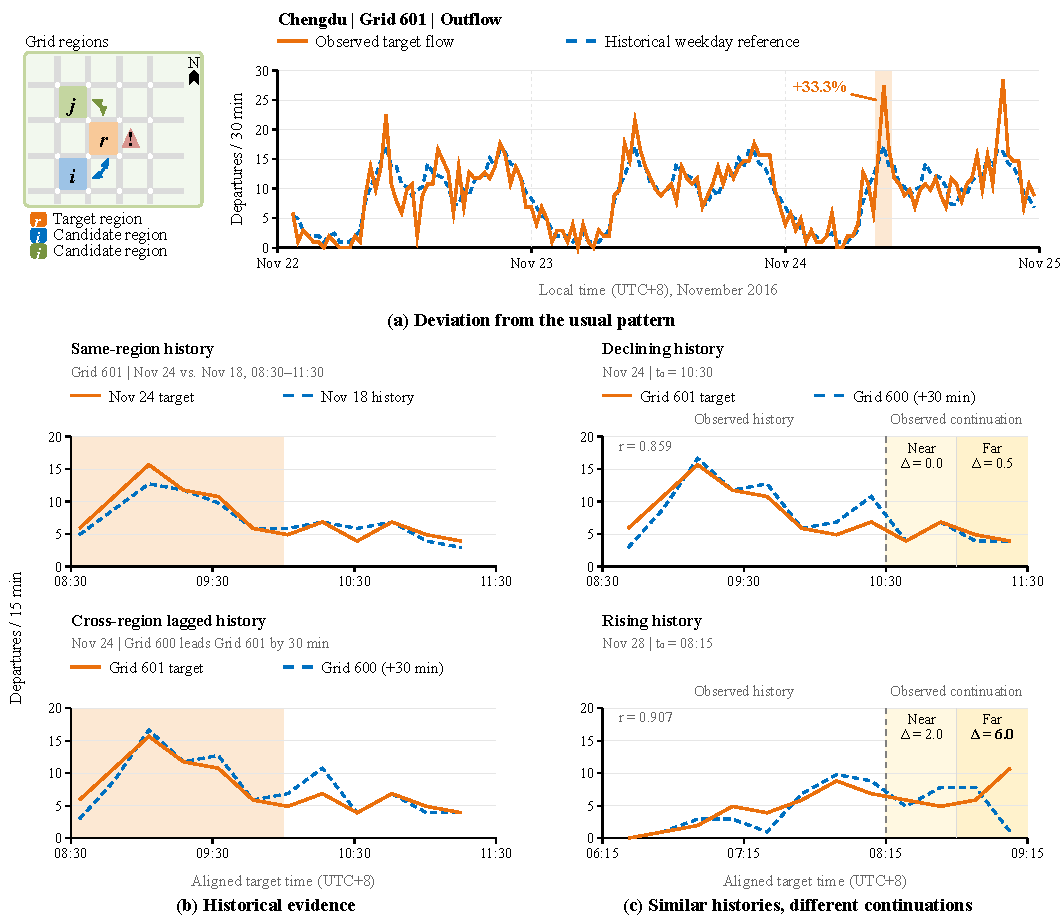
\includegraphics[width=\linewidth]{figures/introduction-case.pdf}
  \caption[常规流量模式偏离与历史信息关联的观测案例]{\textbf{常规流量模式偏离与历史信息关联的观测案例。} 成都2016年11月网格601的流出量，时间均为UTC+8。（a）实测流量与训练期14个工作日同一时段的中位数参照对比；11月24日08:30--10:00的累计流出量高出参照33.3\%，左侧为区域关系示意。（b）同区域11月18日的历史序列及邻网格600提前30分钟的观测；邻区曲线右移30分钟以对齐目标时间。（c）两个案例中，\(r\)为观测截点\(t_0\)前8个15分钟计数的目标与对齐邻区序列之间的Pearson相关系数；Near和Far分别表示\(t_0\)后\([0,30)\)与\([30,60)\)分钟，\(\Delta\)为各区间内两条实测曲线的平均绝对差。（a）按30分钟聚合，（b、c）按15分钟聚合，\(\Delta\)的单位为流出次数/15分钟。案例为事后选取，（c）的后续曲线均为实测观测而非模型预测，Far区间所用邻区源观测发生在\(t_0\)之后。}
  \label{fig:intro-case}
\end{figure}

第一个挑战来自预测证据的异质性。当目标区域偏离常规模式时，可用于修正预测的信息并非来源于单一机制，而是具有明显不同的时间和空间语义。有向时滞关联描述其他区域历史状态与目标区域之间的时间错位关系，而节点自身演化则刻画其局部连续性。这些信息并不是同一种时空依赖的不同强弱形式，而是对应不同的预测角色。若将它们统一压缩到同一种图传播或同一套时序编码中，模型虽然能够学习联合表征，却难以显式保留不同证据的功能差异，也难以进一步形成针对基础预测误差的定向补偿。因此，真正需要解决的问题不是简单地“融合更多信息”，而是如何依据不同证据的作用机制，为其配置差异化的时间编码与关系支持，并将这些信息组织为具有明确角色的预测修正。

第二个挑战在于跨区域历史信息的参考价值具有显著的条件依赖性。空间邻近或历史相关只能表明两个区域可能存在联系，却不能保证候选区域的任一历史状态都适用于当前预测。事实上，同一个候选区域在不同历史时滞、不同时间尺度下所呈现的模式，其参考价值可能明显不同；而在多步预测中，不同未来时距所需要的历史信息也并不完全一致。因此，跨区域建模不能只回答“哪些节点相关”，还需要进一步回答：在当前流量背景下，应从哪个候选区域、哪个历史时刻和哪个时间尺度提取信息，并针对不同预测步赋予多少权重。如果缺乏这种条件化选择机制，无关甚至不匹配的历史消息可能与有效证据同时进入聚合过程，从而削弱对异常变化的刻画能力。

上述两个问题共同指向本文关注的核心研究问题：当目标区域流量偏离其常规时段模式时，如何联合节点自身近期动态与跨区域历史证据，对基础预测进行分层、选择性的残差修正，从而改善短时多步交通流量预测？ 从这一角度看，本文所需的并不是一个更复杂的统一编码器，而是一种能够在已有时空表征之上，分别完成“证据组织”和“历史消息选择”的多级精炼机制。

为此，本文提出一种级联式多级时空残差网络（Cascaded Multi-level Spatio-temporal Residual Network，CMSRN），通过异质专家的自适应融合与背景条件化的历史消息选择，对基础预测进行互补的残差精炼。框架首先通过共享双频时空编码提取低频与高频表征，生成基础预测；随后，状态证据专家残差精炼模块（SERR）围绕节点自身演化和有向时滞关联构建差异化专家，并依据当前状态分配其修正贡献；背景条件跨区域消息选择模块（BCMS）利用目标与来源区域的低频背景，对高频历史消息进行预测步相关的联合选择。两模块分别读取共享表征，生成的修正量在预测端加性融合，共同完成区域流入与流出的短时多步预测。

本文的主要贡献总结如下：

\begin{enumerate}
	\def\labelenumi{\arabic{enumi}.}
	\item
	提出状态证据驱动的异质角色残差精炼模块 SERR。针对常规模式偏离时预测证据的异质性及其贡献分配问题，SERR 构建自身演化与有向时滞两类互补专家，分别刻画节点自身时序演化与跨区域滞后关联。模块结合共享双频表征、相对常规基线的趋势偏差及短时波动证据，通过状态条件门控，在节点和流量通道层面自适应融合自身预测相对于基础预测的残差与时滞专家的补充修正，并以全局可学习强度调节修正幅度，实现对基础预测的状态条件化精炼。
	\item
	提出背景条件化的联合历史消息选择模块BCMS。针对跨区域历史证据的参考价值随流量背景和预测时距变化的问题，BCMS利用目标区域与来源区域的低频背景调制高频多尺度模式匹配，在固定候选邻域内，针对不同预测步对“邻居---时滞---尺度”组合进行联合评分与加权聚合，使历史消息的选择同时适配双端流量背景与未来预测时距。通过将零消息选项纳入联合归一化，模块进一步自适应调节跨区域历史信息的总体引入程度，为基础预测提供背景条件化、预测步相关的残差补充。
	\item
	在成都和上海数据集上开展系统实验，验证CMSRN的预测性能与残差精炼效果。在与13种代表性基线的总体比较中，CMSRN在两城市的四项流入、流出预测任务上均取得最低AVG12 MAE，相较各任务最强基线降低0.46\%--2.00\%，并在其中三项任务上取得最低AVG12 RMSE。进一步结合独立重训练消融与常规模式偏离情景下的分组分析，考察两类残差通路的作用差异：固定模型诊断显示，自身演化修正在近期快速变化样本中具有更大的平均MAE收益，BCMS修正则在目标与候选区域的背景代理较接近时更有效，为角色化证据组织与背景条件化消息选择提供实验依据。
\end{enumerate}
